\qrchapter{https://forgottenpillar.com/rsc/pl-fp-chapter11}{Osobowość Boga — J. S. White}

W dalszej części przyjrzymy się broszurze Jamesa White’a zatytułowanej „\textit{Osobowość Boga}”. Czytając ten artykuł, zobaczymy, że James White kontynuuje tam, gdzie brat Loughborough zakończył, oraz że rozszerza i pogłębia zrozumienie stojące za pierwszym punktem \emcap{Fundamentalnych Zasad}.

Traktat Jamesa White’a był drukowany wielokrotnie, reklamowany 54 razy i przedrukowany dwukrotnie w czasopiśmie „Review and Herald”. Jego pogląd na temat \emcap{osobowości Boga} był dobrze znany i rozpowszechniony w adwentyzmie. W tej broszurze zobaczymy wyraźną krytykę idei, które Kellogg propagował w \textit{The Living Temple}.

\begin{figure}[hp]
    \centering
    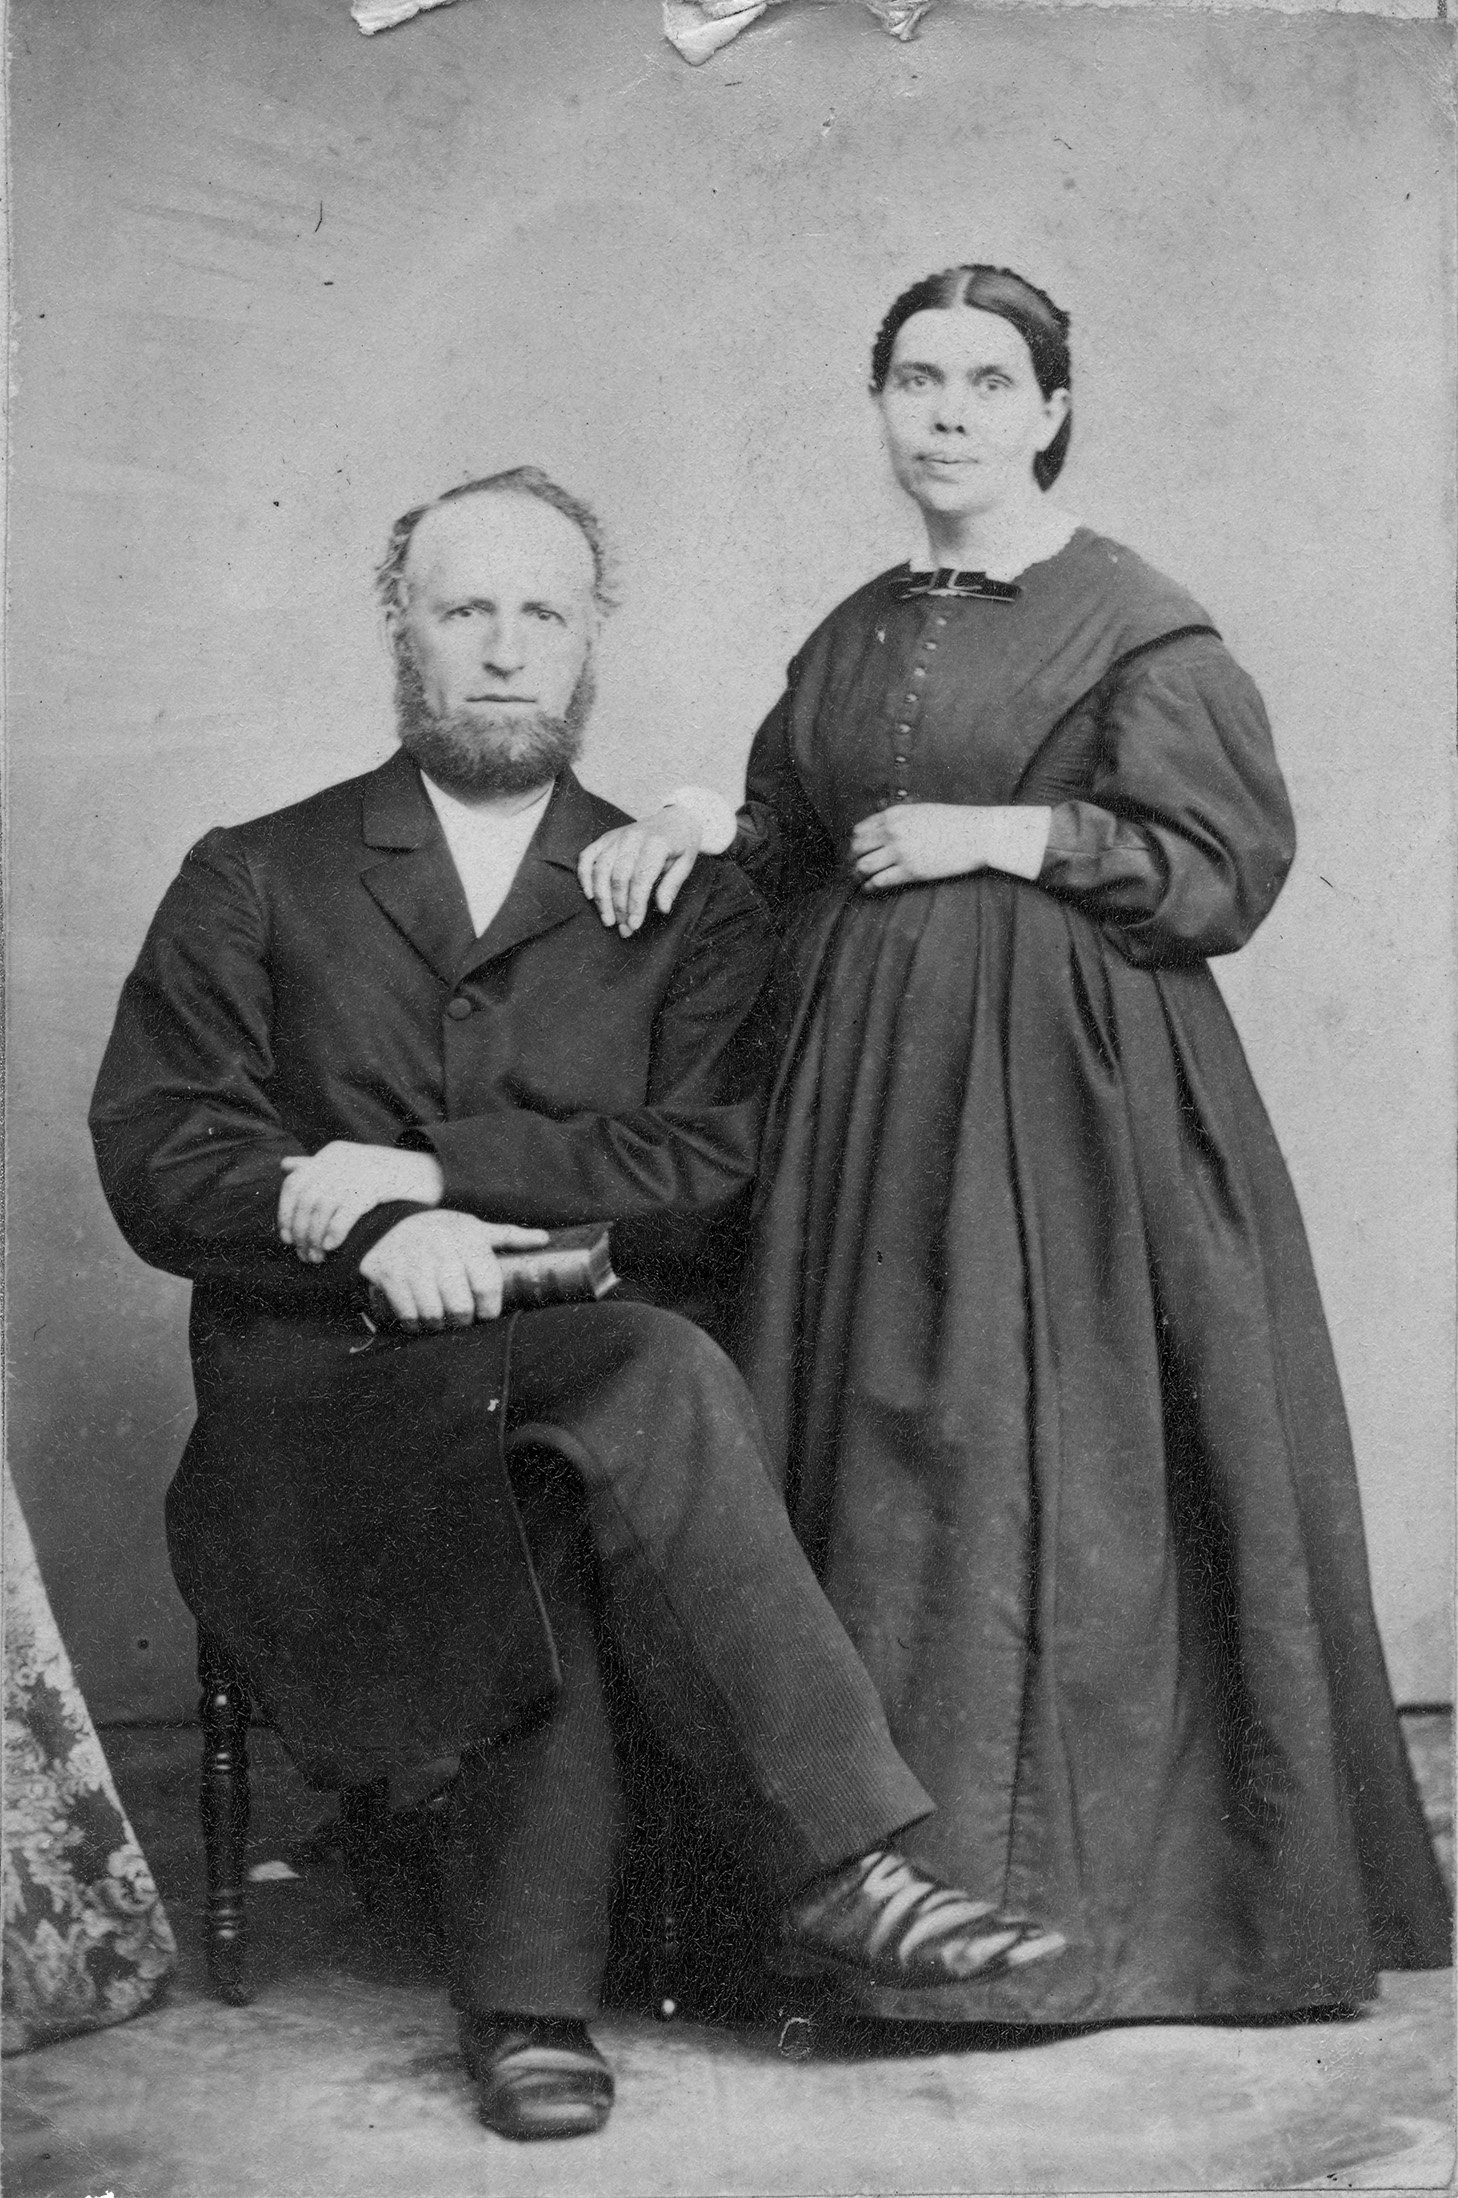
\includegraphics[width=1\linewidth]{images/james-and-ellen-white.jpg}
    \caption*{James Springer White (1821--1881) i Ellen White (1827--1915)}
    \label{fig:james-and-ellen-white}
\end{figure}

\othersQuote{\textbf{CZŁOWIEK został stworzony na obraz Boga}. «I Bóg powiedział: Uczyńmy człowieka na nasz obraz według naszego podobieństwa». «Stworzył więc Bóg człowieka na swój obraz, na obraz Boga go stworzył». Rdz 1:26--27. Patrz także rozdz. 9:6; 1Kor 11:7. \textbf{Ci, którzy zaprzeczają osobowości Boga, mówią, że ‘obraz’ nie oznacza tu \underline{fizycznej postaci}, lecz obraz moralny, i czynią to głównym punktem wyjścia do udowodnienia nieśmiertelności wszystkich ludzi}. Argument przedstawia się następująco: Po pierwsze, człowiek został stworzony na moralny obraz Boga. Po drugie, Bóg jest istotą nieśmiertelną. Po trzecie, zatem wszyscy ludzie są nieśmiertelni. Ale ten sposób rozumowania dowodziłby również, że człowiek jest wszechmocny, wszechwiedzący i wszechobecny, przyodziewając tym samym śmiertelnego człowieka we wszystkie atrybuty boskości. Spróbujmy: Po pierwsze, człowiek został stworzony na moralny obraz Boga. Po drugie, Bóg jest wszechmocny, wszechwiedzący i wszechobecny. Po trzecie, zatem człowiek jest wszechmocny, wszechwiedzący i wszechobecny. To, co dowodzi zbyt wiele, nie dowodzi niczego, dlatego stanowiska, że obraz Boga oznacza Jego moralny obraz, nie da się obronić. \textbf{Jako dowód na to, że Bóg jest osobą, przeczytajmy Jego własne słowa do Mojżesza}: «I Pan rzekł: Oto miejsce przy mnie, a ty staniesz na skale; i stanie się, gdy będzie przechodzić moja chwała, że postawię cię w rozpadlinie skalnej i \textbf{zakryję cię swoją ręką}, kiedy \textbf{będę przechodził}. Potem \textbf{swoją rękę} i \textbf{ujrzysz moje plecy}, lecz \textbf{moje oblicze nie będzie widziane}». Wj 33:21--23. Patrz także rozdz. 24:9--11. \textbf{Tutaj Bóg mówi Mojżeszowi, że \underline{zobaczy Jego postać}}. \textbf{Twierdzenie, że Bóg sprawił, iż Mojżeszowi wydawało się, że widzi Jego postać, podczas gdy On nie ma postaci, jest oskarżaniem Boga o dodanie do fałszu pewnego rodzaju kuglarskiego oszustwa wobec swojego sługi Mojżesza}}[J. S. White, PERGO 1.1; 1861][https://egwwritings.org/read?panels=p1471.3]

\othersQuoteNoGap{Lecz sceptyk uważa, że widzi sprzeczność między wersetem 11, który mówi, że Pan rozmawiał z Mojżeszem twarzą w twarz, a wersetem 20, który stwierdza, że Mojżesz nie mógł zobaczyć Jego oblicza. Niech Lb 12:5--8 usunie tę trudność. \textbf{«A Pan zstąpił w słupie obłoku}, stanął u wejścia do namiotu i wezwał Aarona i Miriam, a oni podeszli oboje. I powiedział do nich: Słuchajcie teraz moich słów. Jeśli będzie wśród was prorok, ja, Pan, objawię się mu w widzeniu i będę mówił do niego we śnie. Lecz nie tak jest z moim sługą Mojżeszem, który jest wierny w całym moim domu. \textbf{Z nim będę mówił z ust do ust, to jest \underline{jawnie}}»}[J. S. White, PERGO 2.1; 1861][https://egwwritings.org/read?panels=p1471.6]

\othersQuoteNoGap{Wielki i straszny Bóg zstąpił otoczony obłokiem chwały. \textbf{Ten obłok można było zobaczyć, ale nie oblicze, które posiada blask jaśniejszy niż tysiąc słońc}. W tych okolicznościach Mojżeszowi pozwolono zbliżyć się i \textbf{rozmawiać z Bogiem twarzą w twarz, czy też z ust do ust, to znaczy \underline{jawnie}}}[J. S. White, PERGO 2.2; 1861][https://egwwritings.org/read?panels=p1471.7]

\othersQuoteNoGap{Mówi prorok Daniel: «I patrzyłem, aż postawiono trony, a \textbf{zasiadł Odwieczny}, którego szata była biała jak śnieg, a \textbf{włosy jego głowy jak czysta wełna}; \textbf{jego tron był jak ognisty płomień, a jego koła jak płonący ogień}». Rozdz. 7:9. «Widziałem w nocnych wizjach, a oto ktoś podobny do Syna człowieczego przybył z obłokami nieba, \textbf{przyszedł do Odwiecznego} i \textbf{przyprowadzono go przed niego}. I dano mu panowanie, chwałę i królestwo». Wersety 13--14}[J. S. White, PERGO 2.3; 1861][https://egwwritings.org/read?panels=p1471.8]

\othersQuoteNoGap{Oto wzniosły opis działania \textbf{dwóch osobistości}, mianowicie \textbf{Boga Ojca i Jego Syna Jezusa Chrystusa}. \textbf{Jeśli zaprzeczy się ich osobowości, to w tych cytatach z Księgi Daniela nie ma żadnej wyraźnej myśli}. W związku z tym cytatem przeczytajmy stwierdzenie apostoła, że \textbf{Syn był dokładnym obrazem osoby swojego Ojca}. «Bóg, który w różnych czasach i na różne sposoby przemawiał w przeszłości do ojców przez proroków, w tych ostatecznych dniach przemówił do nas przez swego Syna, którego ustanowił dziedzicem wszystkiego, przez którego też stworzył światy; \textbf{który, będąc blaskiem jego chwały i dokładnym obrazem jego osoby}». Hbr 1:1--3}[J. S. White, PERGO 3.1; 1861][https://egwwritings.org/read?panels=p1471.11]

\othersQuoteNoGap{Dodajemy tu świadectwo Chrystusa. «A sam Ojciec, który mnie posłał, zaświadczył o mnie. Nigdy nie słyszeliście jego głosu \textbf{ani nie widzieliście jego kształtu}». J 5:37. Patrz także Flp 2:6. \textbf{Twierdzenie, że Ojciec nie ma kształtu osoby, wydaje się najbardziej rażącym zaprzeczeniem jasnych słów Pisma}. \\
ZARZUT. — «\textbf{\underline{Bóg jest Duchem}}». J 4:24}[J. S. White, PERGO 3.2; 1861][https://egwwritings.org/read?panels=p1471.12]

\othersQuoteNoGap{ODPOWIEDŹ. — \textbf{Aniołowie też są duchami} [Ps 104:4], jednak ci, którzy odwiedzili Abrahama i Lota, położyli się, jedli i chwycili Lota za rękę. \textbf{Byli istotami duchowymi. Tak samo Bóg jest istotą duchową}}[J. S. White, PERGO 3.3; 1861][https://egwwritings.org/read?panels=p1471.13]

\othersQuoteNoGap{ZARZUT. — \textbf{Bóg jest wszędzie}. Dowód. Ps 139:1--8. \textbf{Jest On tak samo w jednym miejscu, jak w jakimkolwiek innym miejscu}}[J. S. White, PERGO 3.4; 1861][https://egwwritings.org/read?panels=p1471.14]

\othersQuoteNoGap{ODPOWIEDŹ. — 1. \textbf{Bóg jest wszędzie poprzez swoją wszechwiedzę}, jak to widać w przytoczonych powyżej słowach Dawida. Wersety 1--6. «Panie, \textbf{przeniknąłeś mnie i znasz mnie}. \textbf{Wiesz}, kiedy siedzę i wstaję; \textbf{znasz} moje myśli z daleka. Otaczasz moją ścieżkę i mój spoczynek i \textbf{znane} ci są wszelkie moje drogi. Zanim na moim języku pojawi się słowo, oto ty, Panie, już je \textbf{znasz całe}. Otoczyłeś mnie z tyłu i z przodu i położyłeś na mnie swoją rękę. \textbf{Taka wiedza} jest dla mnie zbyt cudowna. Jest wzniosła; nie mogę jej pojąć»}[J. S. White, PERGO 3.5; 1861][https://egwwritings.org/read?panels=p1471.15]

\othersQuoteNoGap{2. \textbf{Bóg jest \underline{wszędzie poprzez swojego Ducha}, \underline{który jest Jego przedstawicielem} i objawia się gdziekolwiek On zechce}, jak to widać w tych samych słowach, na które powołuje się oponent. Wersety 7--10. «\textbf{Dokąd ujdę przed \underline{twoim Duchem}}? Albo \textbf{dokąd ucieknę przed \underline{twoją obecnością}}? Jeśli wstąpię do nieba, jesteś tam; jeśli przygotuję sobie posłanie w piekle, oto tam jesteś; gdybym wziął skrzydła poranka i zamieszkał na krańcu morza, i tam twoja ręka prowadziłaby mnie, a twoja prawica by mnie podtrzymała»}[J. S. White, PERGO 4.1; 1861][https://egwwritings.org/read?panels=p1471.18]

\othersQuoteNoGap{\textbf{Bóg jest w niebie}. Tego uczy nas Modlitwa Pańska. «\textbf{Ojcze nasz, który jesteś w niebie}». Mt 6:9; Łk 11:2. \textbf{Lecz jeżeli Bóg jest tak samo w jednym miejscu, jak w jakimkolwiek innym miejscu, to niebo również jest tak samo w jednym miejscu, jak w jakimkolwiek innym miejscu, a idea pójścia do nieba jest kompletną pomyłką}. Wszyscy jesteśmy w niebie; a Modlitwa Pańska, według tej mglistej teologii, oznacza po prostu: Ojcze nasz, \textbf{który jesteś wszędzie}, niech będzie uświęcone twoje imię. Niech przyjdzie twoje królestwo, niech się dzieje twoja wola na ziemi, \textbf{tak jak wszędzie}}[J. S. White, PERGO 4.2; 1861][https://egwwritings.org/read?panels=p1471.19]

\othersQuoteNoGap{Ponadto czytelnicy Biblii dotąd wierzyli, że Henoch i Eliasz zostali rzeczywiście wzięci \textbf{do Boga w niebie}. \textbf{Lecz jeśli Bóg i niebo są tak samo w jednym miejscu, jak w jakimkolwiek innym miejscu, to jest to całkowitą pomyłką}. Nie zostali oni przeniesieni. A cała ta historia o ognistym rydwanie, ognistych koniach i towarzyszącym temu wichrze, który zabrał Eliasza do nieba, była bezużytecznym widowiskiem. Oni po prostu wyparowali, a mglista para przeszła przez cały wszechświat. To wszystko, co umysł może pojąć o Henochu i Eliaszu, \textbf{jeżeli przyjmie, że Bóg i niebo nie są bardziej w jakimś pojedynczym miejscu niż wszędzie}. Jednak o Eliaszu jest napisane, że «\textbf{wstąpił} wśród wichru \textbf{do nieba}». 2Krl 2:11. A o Henochu jest napisane, że «chodził z Bogiem i go nie było, bo Bóg go zabrał». Rdz 5:24}[J. S. White, PERGO 4.3; 1861][https://egwwritings.org/read?panels=p1471.20]

\othersQuoteNoGap{\textbf{Jest powiedziane, że Jezus jest po prawicy Majestatu na wysokościach}. Hbr 1:3. «A po tym, jak Pan do nich przemówił, \textbf{został \underline{wzięty do nieba}} \textbf{i zasiadł po prawicy Boga}». Mk 16:19. \textbf{Ale jeśli niebo jest wszędzie i Bóg jest wszędzie, to wniebowstąpienie Chrystusa do prawicy Ojca oznacza po prostu, że udał się wszędzie}! Został uniesiony tylko tam, gdzie obłok ukrył go przed wzrokiem uczniów, a potem wyparował i udał się wszędzie! Tak więc zamiast ukochanego Jezusa, tak pięknie opisanego w obu Testamentach, mamy tylko pewien rodzaj oparów rozproszonych po całym wszechświecie. A zgodnie z tą rozproszoną teologią powtórne przyjście Chrystusa, czyli Jego powrót, byłby kondensacją tych oparów w jakimś miejscu, na przykład na Górze Oliwnej! \textbf{Chrystus powstał z martwych w fizycznej postaci}. «Nie ma go tu», powiedział anioł, «powstał bowiem, jak powiedział». Mt 28:6}[J. S. White, PERGO 5.1; 1861][https://egwwritings.org/read?panels=p1471.23]

\othersQuoteNoGap{«A kiedy szły opowiedzieć to jego uczniom, oto Jezus wyszedł im na spotkanie, mówiąc: Bądźcie pozdrowione! A one podeszły, \textbf{objęły go za nogi} i oddały mu pokłon». Werset 9}[J. S. White, PERGO 5.2; 1861][https://egwwritings.org/read?panels=p1471.24]

\othersQuoteNoGap{«\textbf{Popatrzcie na moje ręce i stopy}», powiedział Jezus do tych, którzy wątpili w Jego zmartwychwstanie, «że to jestem ja sam. \textbf{Dotknijcie mnie i zobaczcie, \underline{bo duch nie ma ciała ani kości}, jak widzicie, że ja mam}. I kiedy to powiedział, \textbf{pokazał im ręce i stopy}. A gdy oni jeszcze nie wierzyli z radości i dziwili się, zapytał ich: Macie tu coś do jedzenia? I podali mu kawałek pieczonej ryby i plastra miodu, a on wziął i jadł przed nimi». Łk 24:39--43}[J. S. White, PERGO 5.3; 1861][https://egwwritings.org/read?panels=p1471.25]

\othersQuoteNoGap{Po tym, jak Jezus przemówił do swoich uczniów na Górze Oliwnej, \textbf{został uniesiony od nich}, a obłok zabrał go sprzed ich oczu. «A gdy patrzyli uważnie \textbf{w niebo, jak wstępował}, oto stanęli przy nich dwaj mężowie w białych szatach, którzy powiedzieli: Mężowie z Galilei, dlaczego stoicie, patrząc w niebo? Ten Jezus, który \textbf{został od was wzięty w górę do nieba}, przyjdzie tak samo, jak widzieliście go \textbf{wstępującego do nieba}». Dz 1:9--11. J. W.}[J. S. White, PERGO 6.1; 1861][https://egwwritings.org/read?panels=p1471.27]

James White zwalcza ideę, że Bóg jest tylko duchem i jako taki jest obecny \othersnodot{tak samo w jednym miejscu, jak w jakimkolwiek innym miejscu}. Przedstawia jasne i jednoznaczne świadectwo z Pisma Świętego, że Bóg jest osobową istotą; te same poglądy widzimy w pismach Ellen White.

\egw{Potężna moc, która działa w całej przyrodzie i podtrzymuje wszystko, nie jest, jak twierdzą niektórzy ludzie nauki, \textbf{jedynie wszechobecną zasadą}, energią napędową. \textbf{\underline{Bóg jest duchem, ale jest osobową istotą}}, \textbf{gdyż człowiek został stworzony na Jego obraz}. \textbf{Jako \underline{osobowa istota}}, Bóg objawił się w swoim Synu. Jezus, blask chwały Ojca, «i \textbf{dokładny \underline{obraz Jego osoby}}» (Hbr 1:3), na ziemię przyszedł w postaci człowieka. Jako \textbf{osobowy Zbawiciel} przyszedł na świat. Jako \textbf{osobowy Zbawiciel wstąpił \underline{na wysokości}}. Jako \textbf{osobowy Zbawiciel wstawia się \underline{na niebiańskich dworach}}. \textbf{Przed tronem Bożym} w naszym imieniu służy «Podobny do Syna człowieczego». Dn 7:13}[Ed 131.5; 1903][https://egwwritings.org/read?panels=p29.632]

Ellen White i pionierzy adwentyzmu rozróżniali między terminem ‘\textit{duch}’ a ‘\textit{istota}’. Bóg jest osobową istotą, nie tylko duchem. On nie jest \othersnodot{tak samo w jednym miejscu, jak w jakimkolwiek innym miejscu}, ale jest \othersnodot{w jednym miejscu bardziej niż w innym}[J. N. Loughborough, \textit{Is the Soul Immortal? Is God a Person?}, „The Advent Review, and Sabbath Herald”, 18 września 1855, s. 41.][https://documents.adventistarchives.org/Periodicals/RH/RH18550918-V07-06.pdf]. Jest w niebie, w swojej świątyni, siedząc na swoim tronie — osobiście — i jest wszędzie obecny przez swojego przedstawiciela, Ducha Świętego.

Oto kilka innych cytatów z siostry White, które są w harmonii z poglądami pionierów na temat \emcap{osobowości Boga}:

\egw{On \normaltext{[Jezus]} nauczał, że Bóg nagradza sprawiedliwych i karze przestępców. \textbf{Nie był On niematerialnym duchem}, ale żywym władcą wszechświata. \textbf{Ten łaskawy Ojciec} nieustannie działał dla dobra człowieka i troszczył się o wszystko, co go dotyczy}[3SP 47.1; 1878][https://egwwritings.org/read?panels=p142.195]

\egw{\textbf{Biblia ukazuje nam \underline{Boga w Jego wysokim i świętym miejscu}}, nie w stanie bezczynności, nie w ciszy i samotności, ale otacza Go dziesięć tysięcy razy dziesięć tysięcy i tysiące tysięcy świętych istot, wszystkie gotowe wypełniać Jego wolę. \textbf{Poprzez tych posłańców aktywnie komunikuje się z każdą częścią swojego królestwa}. \textbf{\underline{Przez swojego Ducha jest wszędzie obecny}}. \textbf{Poprzez działanie swojego Ducha i swoich aniołów} służy dzieciom ludzkim}[MH 417.2; 1905][https://egwwritings.org/read?panels=p135.2136]

\egw{Wielkość Boga jest dla nas niepojęta. «\textbf{Tron Pana jest w niebie}» (Ps 11:4); \textbf{\underline{jednak przez swojego Ducha jest On wszędzie obecny}}. \textbf{Ma On dokładną wiedzę} o wszystkich dziełach swoich rąk i osobiście się nimi interesuje}[Ed 132.2; 1903][https://egwwritings.org/read?panels=p29.636]

\egw{Przez Jezusa Chrystusa \textbf{Bóg — nie wonności, \underline{nie coś nieuchwytnego}, \underline{ale osobowy Bóg}} — stworzył człowieka i obdarzył go inteligencją i mocą}

Dalej w broszurze Jamesa White'a czytamy jego ostrą krytykę pojęcia niematerialnego Boga. Wcześniej przypomnijmy krótko argument dr. Kellogga, że \othersnodot{\textbf{\underline{dyskusje dotyczące postaci Boga są całkowicie bezużyteczne}}}, ponieważ Bóg jest \othersnodot{\textbf{daleko poza naszym pojmowaniem \underline{jak granice przestrzeni i czasu}}}. Wierzył on, że osoba Boga nie jest ograniczona do jednego miejsca, ponieważ jest On \othersnodot{tak samo w jednym miejscu, jak w jakimkolwiek innym miejscu}\footnote{W \textit{The Living Temple} dr Kellogg zaprzecza temu, że Bóg może być obecny wszędzie naraz: „\textit{Ktoś powie}: «Bóg może być obecny przez swojego Ducha lub przez swoją moc, ale z pewnością sam Bóg \textit{nie może być obecny wszędzie naraz}». Odpowiadamy: Jak można oddzielić moc od źródła mocy? Gdzie Duch Boży działa, gdzie moc Boża się objawia, tam sam Bóg jest \textit{rzeczywiście i prawdziwie obecny}”. \href{https://archive.org/details/J.H.Kellogg.TheLivingTemple1903/page/n29/}{J. H. Kellogg, \textit{The Living Temple}, Good Health Publishing Company, Battle Creek, Mich. 1903, s. 28.}}. Gdyby Bóg w swojej osobowości był naprawdę konkretną istotą, posiadającą namacalne ciało, to nie byłby w stanie być obecny \othersnodot{tak samo w jednym miejscu, jak w jakimkolwiek innym miejscu}, a tym samym podtrzymywać życie. W dalszej części James White pisze przeciwko rozumowaniu, że Bóg jest niematerialny w swojej osobie.

\othersQuoteNoDot{NIEMATERIALNOŚĆ}

\othersQuoteNoGap{\textbf{TO jest jedynie inne określenie nicości}. \textbf{Jest to zaprzeczenie wszystkich} \textbf{rzeczy i \underline{istot}} — całego istnienia. Nie ma ani jednego dowodu potwierdzającego jej istnienie. Nie ma sposobu, by mogła się objawić jakiejkolwiek inteligencji w niebie czy na ziemi. \textbf{Ani Bóg, ani aniołowie, ani ludzie nie mogliby pojąć takiej substancji, istoty czy rzeczy}. \textbf{Nie posiada ona żadnej właściwości ani mocy, przez którą \underline{mogłaby się objawić jakiejkolwiek inteligentnej istocie} we wszechświecie}. Rozum i analogia nigdy jej nie badają ani nawet nie pojmują. \textbf{Objawienie nigdy jej nie ujawnia ani żaden z naszych zmysłów nie świadczy o jej istnieniu}. \textbf{Nie można jej zobaczyć, poczuć, usłyszeć, posmakować ani powąchać, nawet przy najsilniejszych organach czy najbardziej wyczulonych zmysłach}. Nie jest ani płynna, ani stała, miękka, ani twarda — nie może się ani rozszerzać, ani kurczyć. Krótko mówiąc, nie może wywierać żadnego wpływu — nie może ani działać, ani być przedmiotem działania. A nawet jeśli istnieje, nie może być w żaden sposób użyteczna. Nie posiada ani jednej pożądanej właściwości, zdolności czy zastosowania, jednak, co dziwne, \textbf{niematerialność jest Bogiem współczesnego chrześcijanina}, \textbf{jego oczekiwanym niebem}, \textbf{jego nieśmiertelnym ja} — \textbf{jego wszystkim}!}

\othersQuoteNoGap{\textbf{O sekciarstwo! O ateizm!! O unicestwienie!!!} \textbf{Kto może dostrzec subtelne różnice między jednym a drugim?} Wydają się podobne, różnią się tylko nazwą. \textbf{Według ateisty nie ma Boga. \underline{Według sekciarza jest Bóg bez ciała i części}.} Kto może określić różnicę? Z naszej strony nie dostrzegamy różnicy nawet o włos; \textbf{oba poglądy negują wszystko, co istnieje} — i obydwa są pozbawione mocy i poznania}[J. S. White, PERGO 6.3; 1861][https://egwwritings.org/read?panels=p1471.30]

\othersQuoteNoGap{\textbf{Według ateisty nie ma życia po śmierci ani świadomego istnienia po grobie. Sekciarz ma, \underline{lecz jest ono niematerialne jak jego Bóg, i bez ciała czy części}. Tutaj znowu oba poglądy są przeczące i obydwa prowadzą do tego samego punktu}. Wiarę i nadzieję sprowadzają do tego samego, tylko wyrażonego innymi terminami}[J. S. White, PERGO 7.1; 1861][https://egwwritings.org/read?panels=p1471.33]

\othersQuoteNoGap{Co więcej, \textbf{według ateisty nie ma nieba w wieczności}. \textbf{Według sekciarz jest niebo, ale jest ono \underline{niematerialne we wszystkich swoich właściwościach}, i dlatego jest negacją wszelkich bogactw i substancji}. Tutaj znowu dwa poglądy są równoznaczne i prowadzą do tego samego punktu}[J. S. White, PERGO 7.2; 1861][https://egwwritings.org/read?panels=p1471.34]

\othersQuoteNoGap{Ponieważ nie zazdrościmy im posiadania wszystkiego, co sobie roszczą, pozwolimy im teraz się tym cieszyć w spokoju i bez przeszkód i przejdziemy do zbadania części, którą może nadal cieszyć się znienawidzony materialista}[J. S. White, PERGO 7.3; 1861][https://egwwritings.org/read?panels=p1471.35]

\othersQuoteNoGap{\textbf{Czym jest Bóg? Jest On materialną, uporządkowaną duchową istotą, \underline{posiadającą zarówno ciało, jak i części}. Człowiek powstał na Jego obraz}}[J. S. White, PERGO 7.4; 1861][https://egwwritings.org/read?panels=p1471.36]

\othersQuoteNoGap{\textbf{Czym jest Jezus Chrystus? Jest Synem Bożym i jest \underline{jak Jego Ojciec}, to znaczy «blaskiem chwały Ojca i dokładnym obrazem Jego osoby». \underline{Jest On materialną istotą duchową, z ciałem, częściami} i uczuciami; posiadającą nieśmiertelne ciało i nieśmiertelne kości}}[J. S. White, PERGO 7.5; 1861][https://egwwritings.org/read?panels=p1471.37]

\othersQuoteNoGap{\textbf{Czym są ludzie?} Są potomstwem Adama. \textbf{Są zdolni do otrzymywania wiedzy i wywyższenia w takim stopniu, aby zostali \underline{wskrzeszeni z martwych z ciałem jak ciało Jezusa Chrystusa} \underline{i posiedli nieśmiertelne ciało i kości}}. W ten sposób doprowadzeni do doskonałości, posiądą \textbf{materialny wszechświat}, czyli ziemię, jako swoje «wieczne dziedzictwo». Mając przed sobą te nadzieje i perspektywy, mówimy chrześcijańskiemu światu, który wyznaje niematerialność, że mogą zachować swojego Boga — swoje życie — swoje niebo i wszystko inne. Roszczą sobie prawo tylko do tego, co my odrzucamy; a my rościmy sobie prawo tylko do tego, co oni odrzucają. \textbf{Dlatego nie ma podstaw do kłótni czy sporu między nami}}[J. S. White, PERGO 7.6; 1861][https://egwwritings.org/read?panels=p1471.38]

\othersQuoteNoGap{Dla nas materia — a nie-obiekty \\
Niech sobie biorą mistyczne sekty; \\
Kto czego chce, niech przy tym trwa \\
I niezmąconą radość ma. \\
Oni chcą Boga mieć bez ciała, \\
Lecz dla nas taki Bóg nie działa; \\
\textbf{Też niby-piekła nam nie trzeba,} \\
\textbf{Chcemy materialnego nieba.} \\
\textbf{My ziemię, niebo, gwiazdy znamy,} \\
\textbf{Powietrze, którym oddychamy;} \\
\textbf{Złoto i srebro, kosztowności,} \\
\textbf{A także ciała z krwi i kości.} \\
\textbf{Nadzieja nasza wciąż ta sama,} \\
\textbf{Po odjęciu winy Adama} \\
\textbf{Wszystko już będzie dla człowieka,} \\
\textbf{A on dla Pana na wiek wieka}}[J. S. White, PERGO 8.1; 1861][https://egwwritings.org/read?panels=p1471.41]

James White porównał poglądy o niematerialnym Bogu do sekciarstwa, ateizmu i anihilacjonizmu. „\textit{Niematerialny Bóg}” jest innym wyrażeniem na nieistnienie Boga. James White nigdy nie otrzymał żadnej nagany od siostry White za te poglądy; przeciwnie, były one popierane przez jej pisma. Wielu twierdzi, że siostra White zmieniła swoje poglądy z czasem i później przyjęła doktrynę o Trójcy, ale nie jest to poparte dokładnymi zapisami historycznymi. W 1905 roku siostra White wspomina spotkanie z dr. Kelloggiem, kiedy to dwadzieścia lat wcześniej przyszedł do niej z tymi samymi poglądami dotyczącymi \emcap{osobowości Boga}, które James White i inni pionierzy obalali:

\egw{A więc ten temat nie schodził mi sprzed oczu przez ponad dwadzieścia lat. Mój mąż nie żyje od dwudziestu lat, a przed jego śmiercią wkradły się pewne rzeczy. Dr Kellogg przyszedł do mojego pokoju; zajmowałam jeden z dużych pokoi w biurze jako mój dom. Miałam tam dwa lub trzy pokoje, i \textbf{otrzymał wielkie światło}; i usiadł i powiedział, jakie było jego światło: \textbf{to są dokładnie te same teorie czy błędy, te same sofizmaty, które przedstawia i przedstawiał w «The Living Temple».} Powiedziałam: «Dr. Kelloggu, \textbf{już się z tym spotkałam}». Spotkałam się z tym, gdy po raz pierwszy zaczęłam podróżować. Spotkałam się z tym na Północy; spotkałam się z tym w New Hampshire. Widziałam przekleństwo tego wpływu w Massachusetts i \textbf{świadectwa, które mi dano, mówiły wprost, że nie możemy czegoś takiego nauczać w naszych kościołach}. I rozmawiałam z nim. \textbf{Przedstawiłam historię} — nie mam czasu, żeby przedstawić ją tutaj. \textbf{Przedstawiłam mu historię o tym, jak Duch Boży to traktował i jak my jako lud musimy uniknąć tych sofizmatów i złudzeń}. I to kaznodzieje zwodzili ludzi tymi sofizmatami. \textbf{Nie powiem wam, do czego to prowadziło} — \textbf{może to musi nadejść}; ale nie powiem wam teraz, do czego to prowadziło; \textbf{ale powiem wam, do czego prowadzą te sofizmaty:} \textbf{prowadzą do \underline{nieistnienia Chrystusa, do nieistnienia Boga}, \underline{Jego osobowości}, i wprowadzają — jak to nazwać? — pewien rodzaj \underline{sfabrykowanej teorii o Bogu i Chrystusie}}}[Ms70a-1905.11; 1905][https://egwwritings.org/read?panels=p12696.17]

Poglądy Kellogga w \textit{The Living Temple} dotyczące \emcap{osobowości Boga} prowadzą do nieistnienia Chrystusa i nieistnienia Boga. Dlaczego? Ponieważ jego poglądy o Bogu zakładają niematerialnego Boga. Kościół mierzył się z takimi poglądami na początku swojej działalności. James White pisał o nich w swojej broszurze \textit{The Personality of God}, a siostra White przypominała te wczesne doświadczenia, gdy wraz z mężem zwalczali błąd, że Bóg jest niematerialnym, wszechogarniającym duchem.

% ignore
